\documentclass{beamer}
%
% Choose how your presentation looks.
%
% For more themes, color themes and font themes, see:
% http://deic.uab.es/~iblanes/beamer_gallery/index_by_theme.html
%
\mode<presentation>
{
  \usetheme{Madrid}      % or try Darmstadt, Madrid, Warsaw, ...
  \usecolortheme{default} % or try albatross, beaver, crane, ...
  \usefonttheme{default}  % or try serif, structurebold, ...
  \setbeamertemplate{navigation symbols}{}
  \setbeamertemplate{caption}[numbered]
}

\usepackage[english]{babel}
\usepackage[utf8x]{inputenc}
\usepackage{graphicx}
\usepackage{array}

\title[16-threads]{EA879 -- Introdução ao Software
Básico\\}
\author{Tiago F. Tavares}
\institute{FEEC -- UNICAMP}
\date{Aula 16 -- 24/outubro/2018}

\begin{document}

\begin{frame}
  \titlepage
\end{frame}

% Uncomment these lines for an automatically generated outline.
%\begin{frame}{Outline}
%  \tableofcontents
%\end{frame}

\section{Introdução}

\begin{frame}{Objetivos}
  \Large
  \begin{itemize}
    \item Identificar condições de deadlock em código
    \item Enumerar as condições que levam a deadlock
    \item Analisar soluções para deadlock
  \end{itemize}
\end{frame}

\begin{frame}[fragile]{Previously, on EA879...}
  \centering
  \Large
  \begin{itemize}
  \item Procesos
  \item Pipes
  \item Preempção
  \item Fork
  \item Memória compartilhada
  \item Dispatchers
  \item Produtor-consumidor
  \item Threads
  \item Mutexes
  \end{itemize}
\end{frame}

\begin{frame}[fragile]{Revisão}
  \centering
  \Large
  Qual é a diferença entre uma thread e um processo?
\end{frame}

\begin{frame}[fragile]{Revisão}
  \centering
  \Large
  Qual é a utilidade de um mutex em uma thread?
\end{frame}

\begin{frame}[fragile]{Exercício}
  \centering
  \Large
  Exercício 1
\end{frame}

\begin{frame}[fragile]{Hm...}
  \centering
  \LARGE
  O que saiu errado?
  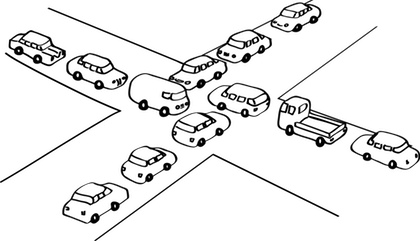
\includegraphics[width=0.7\textwidth]{deadlock1.jpeg}
\end{frame}


\begin{frame}[fragile]{Deadlock}
  \centering
  \LARGE
  DEADLOCK!\\
  
\includegraphics[width=0.7\textwidth]{evil_deadlock.jpg}
\end{frame}

\begin{frame}[fragile]{Deadlock}
  \centering
  \LARGE
  DEADLOCK!\\
  
\includegraphics[width=0.7\textwidth]{dead-lock-cover.jpg}
\end{frame}

\begin{frame}[fragile]{Deadlock}
  \centering
  \LARGE
  DEADLOCK!\\
  
\includegraphics[width=0.5\textwidth]{Deadlock2.jpg}
\end{frame}

\begin{frame}[fragile]{Deadlock}
  \centering
  \Large
  Na computação...\\
  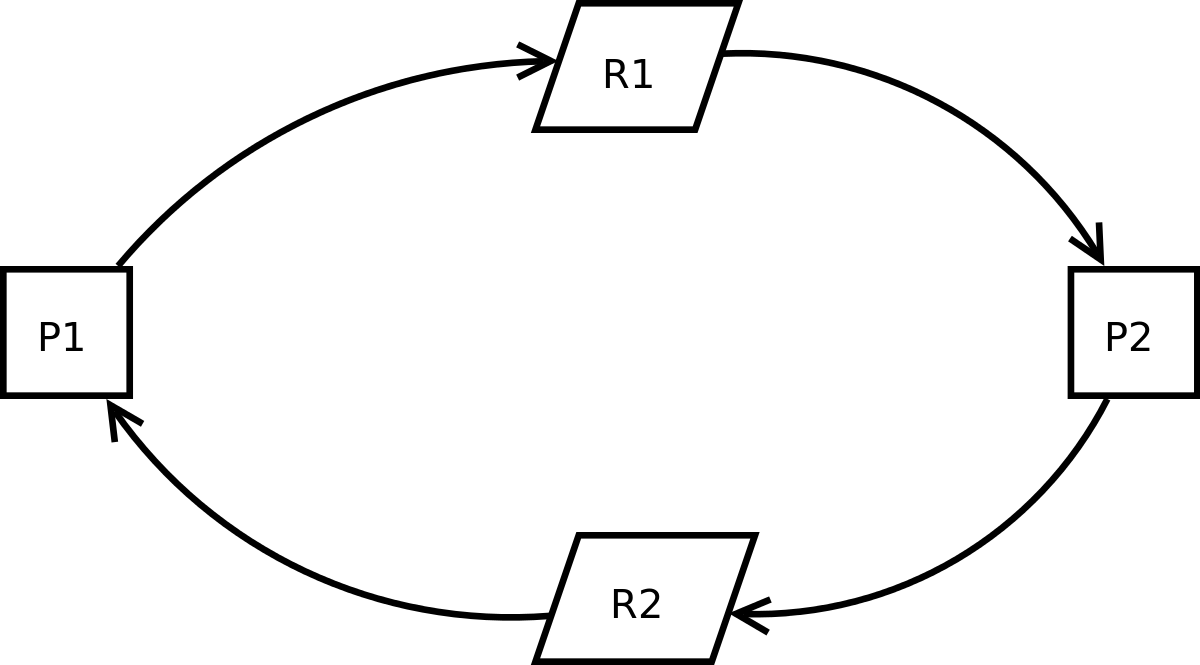
\includegraphics[width=0.7\textwidth]{deadlock_processos.png}
\end{frame}

\begin{frame}[fragile]{Exercício}
  \centering
  \Large
  Exercício 2
  \begin{enumerate}
    \item <2-> \textsc{pthread\_mutex\_trylock()} não trava o programa até que
      a trava seja liberada. Ao invés disso, retorna imediatamente o status de
      erro referente a ter conseguido ou não a trava.
  \end{enumerate}
\end{frame}

\begin{frame}[fragile]{Exercício}
  \centering
  \Large
  Exercício 3
  \begin{enumerate}
    \item <2-> Quanto trabalho adicional o programador tem que ter
      ao projetar cada função (medir em linhas de código)?
    \item <2-> Quanto tempo uma thread teria que ficar em espera, em média
      (estimar usando a linha do tempo)?
  \end{enumerate}
\end{frame}


\begin{frame}[fragile]{Exercício}
  \centering
  \Large
  Exercício 4
  \begin{enumerate}
    \item <2-> Força bruta: mutex mais amplo
    \item <2-> Espera mais longa: random sleep
    \item <2-> Programação cuidadosa: método altruista
  \end{enumerate}
\end{frame}

\begin{frame}[fragile]{Exercício}
  \centering
  \Large
  Exercício 5
  \begin{enumerate}
    \item <2-> \textsc{Exclusão mútua / não-preempção}: parte da implementação
      do Mutex.
    \item <3-> \textsc{Posse-e-espera}: lock na trava1 e depois espero lock na
      trava2 (e vice versa)
    \item <4-> \textsc{Espera circular}: thread1 tem trava1 e quer trava2;
      thread2 tem trava2 e quer trava1.
  \end{enumerate}
\end{frame}


\begin{frame}[fragile]{Exercício}
  \centering
  \Large
  Exercício 6
  \begin{enumerate}
    \item <2-> Altruista: reduz condição de posse-e-espera.
    \item <3-> Força bruta: reduz condição de espera circular.
    \item <4-> Espera dupla: reduz chances de ocorrer espera circular.
  \end{enumerate}
\end{frame}


\begin{frame}[fragile]{Revisão}
  \centering
  \Large
  \begin{enumerate}
    \item Em que situações mutexes devem ser usados em threads?
    \item Como eles podem causar travamentos no programa?
  \end{enumerate}
\end{frame}

\end{document}
